%%%%%%%%%%%%%%%%%%%%%%%%%%%%%%%%%%%%%%%%%%%%%%%%%%%%%%%
% Severity Cheat Sheet
%
% Created by Stephen J Mildenhall
% (c) 2023
%
%%%%%%%%%%%%%%%%%%%%%%%%%%%%%%%%%%%%%%%%%%%%%%%%%%%%%%%

\documentclass{article}

% general includes
\usepackage[landscape]{geometry}
\usepackage{url}
\usepackage{multicol}
\usepackage{amsmath}
\usepackage{amsfonts}
\usepackage{tikz}
\usepackage{xcolor}
% \usetikzlibrary{decorations.pathmorphing}
\usetikzlibrary{calc}
\usepackage{amsmath}
\usepackage{amssymb}

\usepackage{colortbl}
\usepackage{xcolor}
\usepackage{mathtools}
\usepackage{amsmath,amssymb}
\usepackage{enumitem}

\usepackage[english]{babel}

% fonts
\usepackage{stix}

% for the date/time footer
% \usepackage{datetime}
% \newdateformat{dateandtime}{\THEYEAR-\THEMONTH-\THEDAY at \currenttime}
% \usepackage[calc,useregional,showseconds]{datetime2}
\usepackage{datetime2}


\advance\topmargin-.8in
\advance\textheight3in
\advance\textwidth3in
\advance\oddsidemargin-1.5in
\advance\evensidemargin-1.5in
\parindent0pt
\parskip2pt
\newcommand{\hr}{\centerline{\rule{3.5in}{1pt}}}

% colors from the logo
% https://color.adobe.com/mythemes?viewTheme
\definecolor{highlightcolora}{HTML}{73171F}
\definecolor{highlightcolorb}{HTML}{CB7C13}
\definecolor{highlightcolorc}{HTML}{168C6B}
\definecolor{highlightcolord}{HTML}{355078}
\definecolor{highlightcolore}{HTML}{263940}

\colorlet{washedcolora}{highlightcolora!20!white}
\colorlet{washedcolorb}{highlightcolorb!20!white}
\colorlet{washedcolorc}{highlightcolorc!20!white}
\colorlet{washedcolord}{highlightcolord!20!white}
\colorlet{washedcolore}{highlightcolore!20!white}

\colorlet{texta}{white}
\colorlet{textb}{white}
\colorlet{textc}{white}
\colorlet{textd}{white}
\colorlet{texte}{white}

% circles for method and static method
\definecolor{hred}{rgb}{1, 0.5, 0.5}
\definecolor{hblue}{rgb}{0.5, 0.5, 1}
\newcommand{\m}{% method
\tikz[baseline=(char.base)]{
    \node[circle, fill=hred, text=white, inner sep=1pt, minimum size=1em] (char) {m};
}\;}
\newcommand{\s}{% static method
\tikz[baseline=(char.base)]{
    \node[circle, fill=hblue, text=white, inner sep=1pt, minimum size=1em] (char) {s};
}\;}


%% TikZ MACROS

% title box - adjust text color as appropriate here
\tikzstyle{fancytitle} =[
    fill=highlightcolor,
    text=textcolor,
    font=\bfseries,
    right=10pt
    ]

% content box
\tikzstyle{mybox} = [
    draw=highlightcolor,
    fill=washedcolor,
    very thick,
    rectangle,
    inner sep=10pt,
    inner ysep=10pt
    ]

\newcommand{\addlogo}{
\includegraphics[width=0.75in,height=0.75in,keepaspectratio]{../docs/_static/agg_logo.png}}

\newcommand{\makefooter}{%
% \vfil
% \hfill
\begin{tikzpicture}[remember picture, overlay]
    \node[anchor=south east, inner sep=0pt, outer sep=0pt] at ($(current page.south east) + (-0.125in,0.125in)$) {

        \begin{tikzpicture}
        \node [font=\small, text height=0.75in, align=right, minimum height=0.75in, inner xsep=5pt, inner ysep=0pt] (box){%
            \texttt{aggregate v.0.18.0} \\
            Confidence and precision meets  \\
            ease of use in actuarial analysis \\
            \copyright\ Stephen J Mildenhall \\
            % \dateandtime\today \\
            \DTMnow
        };
        \node[inner sep=0pt, anchor=north west] at (box.north east) {
            \addlogo
        };
        \end{tikzpicture}

    };
\end{tikzpicture}
}

\title{Severity Cheat Sheet}

% color scheme defeined here - just change the suffixes
\colorlet{highlightcolor}{highlightcolorb}
\colorlet{washedcolor}{washedcolorb}
\colorlet{textcolor}{textb}

\begin{document}

{\huge{\textbf{\texttt{Severity} Class Cheat Sheet}}}

\raggedright % The \texttt{Severity} call signature,  \\
\texttt{\m Severity(name, sev\_name="", sev\_a=np.nan, sev\_b=0, sev\_mean=0, sev\_cv=0, sev\_loc=0, sev\_scale=0,} \\
\texttt{\phantom{\m Severity(}sev\_xs=None, sev\_ps=None, sev\_wt=1, sev\_lb, sev\_ub, sev\_conditional=True) }\\

The following tables show all \texttt{\m methods}, and fields or properties (used interchangeably). Comments elucidate the meaning of more obscure entries.


\begin{multicols*}{3}


%------------1. SPECIFICATION & CREATION ---------------
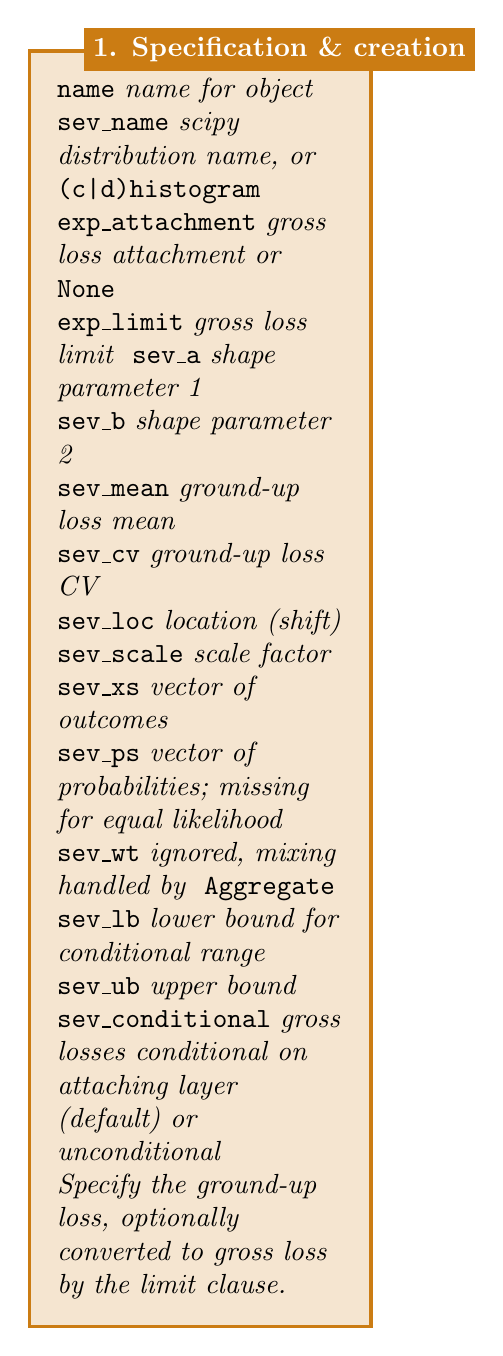
\begin{tikzpicture}
\node [mybox] (box){%
    \begin{minipage}{0.3\textwidth}\raggedright
% {\it italics stuff} \\

\texttt{name} {\it name for object } \\
\texttt{sev\_name} {\it scipy distribution name, or  } \texttt{(c|d)histogram} \\
\texttt{exp\_attachment} {\it gross loss attachment or} \texttt{None} \\
\texttt{exp\_limit} {\it gross loss limit }
\texttt{sev\_a} {\it shape parameter 1} \\
\texttt{sev\_b} {\it shape parameter 2} \\
\texttt{sev\_mean} {\it ground-up loss mean} \\
\texttt{sev\_cv} {\it ground-up loss CV} \\
\texttt{sev\_loc} {\it location (shift)} \\
\texttt{sev\_scale} {\it scale factor } \\
\texttt{sev\_xs} {\it vector of outcomes} \\
\texttt{sev\_ps} {\it vector of probabilities; missing for equal likelihood} \\
\texttt{sev\_wt} {\it ignored, mixing handled by } \texttt{Aggregate} \\
\texttt{sev\_lb} {\it lower bound for conditional range} \\
\texttt{sev\_ub} {\it upper bound} \\
\texttt{sev\_conditional} {\it gross losses conditional on attaching layer (default) or unconditional} \\

\it Specify the ground-up loss, optionally converted to gross loss by the limit clause.


    \end{minipage}
};
\node[fancytitle, right=10pt] at (box.north west) {1. Specification \& creation};
\end{tikzpicture}


%------------2. UPDATE ---------------
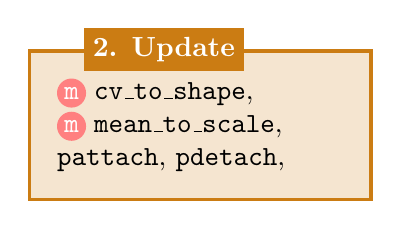
\begin{tikzpicture}
\node [mybox] (box){%
    \begin{minipage}{0.3\textwidth}\raggedright
    
\texttt{\m cv\_to\_shape},
\texttt{\m mean\_to\_scale},
\texttt{pattach},
\texttt{pdetach},


    \end{minipage}
};
\node[fancytitle, right=10pt] at (box.north west) {2. Update};
\end{tikzpicture}


%------------ 3. MOMENTS ---------------
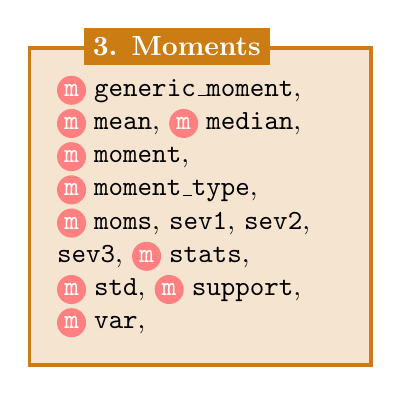
\begin{tikzpicture}
\node [mybox] (box){%
    \begin{minipage}{0.3\textwidth}\raggedright

\texttt{\m generic\_moment},
\texttt{\m mean},
\texttt{\m median},
\texttt{\m moment},
\texttt{\m moment\_type},
\texttt{\m moms},
\texttt{sev1},
\texttt{sev2},
\texttt{sev3},
\texttt{\m stats},
\texttt{\m std},
\texttt{\m support},
\texttt{\m var},


    \end{minipage}
};
\node[fancytitle, right=10pt] at (box.north west) {3. Moments};
\end{tikzpicture}


%------------ 4. STATISTICAL FUNCTIONS ---------------
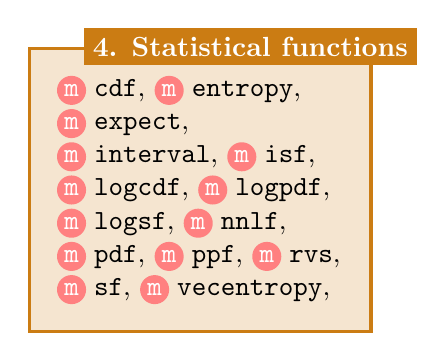
\begin{tikzpicture}
\node [mybox] (box){%
    \begin{minipage}{0.3\textwidth}\raggedright

\texttt{\m cdf},
\texttt{\m entropy},
\texttt{\m expect},
\texttt{\m interval},
\texttt{\m isf},
\texttt{\m logcdf},
\texttt{\m logpdf},
\texttt{\m logsf},
\texttt{\m nnlf},
\texttt{\m pdf},
\texttt{\m ppf},
\texttt{\m rvs},
\texttt{\m sf},
\texttt{\m vecentropy},



    \end{minipage}
};
\node[fancytitle, right=10pt] at (box.north west) {4. Statistical functions};
\end{tikzpicture}


\columnbreak


%------------ 5. VALIDATION ---------------
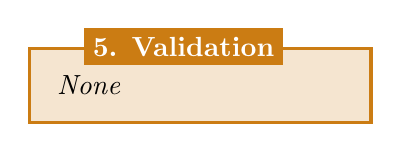
\begin{tikzpicture}
\node [mybox] (box){%
    \begin{minipage}{0.3\textwidth}\raggedright

\it None

    \end{minipage}
};
\node[fancytitle, right=10pt] at (box.north west) {5. Validation};
\end{tikzpicture}


%------------ 6. OUTPUT ---------------
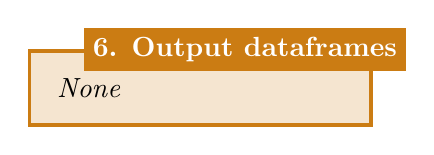
\begin{tikzpicture}
\node [mybox] (box){%
    \begin{minipage}{0.3\textwidth}\raggedright

\it None

    \end{minipage}
};
\node[fancytitle, right=10pt] at (box.north west) {6. Output dataframes};
\end{tikzpicture}


%------------ 7. REINSURANCE ---------------
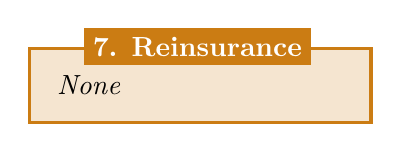
\begin{tikzpicture}
\node [mybox] (box){%
    \begin{minipage}{0.3\textwidth}\raggedright

\it None

    \end{minipage}
};
\node[fancytitle, right=10pt] at (box.north west) {7. Reinsurance};
\end{tikzpicture}


\columnbreak


%------------ 8. VISUALIZTION ---------------
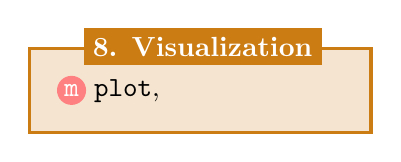
\begin{tikzpicture}
\node [mybox] (box){%
    \begin{minipage}{0.3\textwidth}\raggedright

\texttt{\m plot},


    \end{minipage}
};
\node[fancytitle, right=10pt] at (box.north west) {8. Visualization};
\end{tikzpicture}


%------------ 9. RISK ---------------
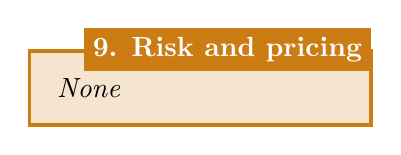
\begin{tikzpicture}
\node [mybox] (box){%
    \begin{minipage}{0.3\textwidth}\raggedright

{\it None }

    \end{minipage}
};
\node[fancytitle, right=10pt] at (box.north west) {9. Risk and pricing};
\end{tikzpicture}


%------------  10. APPROXIMATIONS ---------------
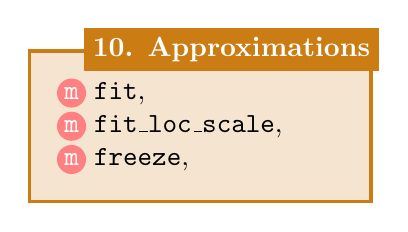
\begin{tikzpicture}
\node [mybox] (box){%
    \begin{minipage}{0.3\textwidth}\raggedright

\texttt{\m fit},
\texttt{\m fit\_loc\_scale},
\texttt{\m freeze},


    \end{minipage}
};
\node[fancytitle, right=10pt] at (box.north west) {10. Approximations};
\end{tikzpicture}


%------------ 11. META ---------------
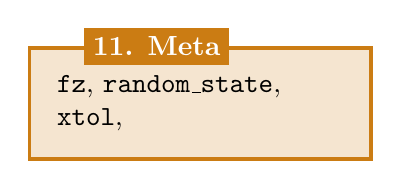
\begin{tikzpicture}
\node [mybox] (box){%
    \begin{minipage}{0.3\textwidth}\raggedright
    
\texttt{fz},
\texttt{random\_state},
\texttt{xtol},

    \end{minipage}
};
\node[fancytitle, right=10pt] at (box.north west) {11. Meta};
\end{tikzpicture}

\bigskip \raggedright
{\bf Notes:} 

[0]: Arguments \texttt{sev\_pick\_attachments=None, sev\_pick\_losses=None, } omitted; see help. 

[1]: matches \texttt{Portfolio} 

Any vectorizable input accepts numeric or iterable datatypes.  

Abbreviations: gcn=gross (subject), ceded, and net; stats: m=mean, cv=coefficient of variation, sd=standard deviation, var=variance, skew(ness); VaR=value-at-risk


% FOOTER
\makefooter

\end{multicols*}

\end{document}
